\documentclass{article}

\usepackage{graphicx}

\begin{document}

\vspace*{3ex}
\begin{flushright}
{\large 3 March 2015}
\end{flushright}

\begin{flushleft}
{\large Jakub Ciecierski\\

}
\end{flushleft}

\hskip3cm

\begin{center}

\Large {\bf
	Cellular automaton
}

\Large {\bf 
	Requirement specification 
}

\vskip2ex


\end{center}

\vskip20ex

\newpage

\section{Goal} 
\Large
\hspace{15pt}The goal of this project is to create an application for cellular automaton. The application 
will allow user to create, save and edit rules and observe new generations on the grid of cells.

\section{Glossary} \par


\setlength{\parindent}{5ex}
\Large {\bf \hspace{15pt} Cellular automaton } - consists of a \textit{grid} of \textit{cells}, each in one of a finite number of \textit{states} (e.g. on and off). 
	A new \textit{generation} is created, according to some fixed
	\textit{rule} that determines the new state of each cell. \\


\Large {\bf 
	Cell 
}	
	- can be in one of many states,
	in case of binary cellular automaton we only have two states for each cell, namely on and off.
	For each cell, a set of cells called its
	\textit{neighborhood} is defined relative to that cell.	\\


\Large {\bf 
	Grid
} 	
	- can be in any finite number of dimensions. Consists of cells.
	An initial state is selected by assigning a state for each cell \\


\Large {\bf Rule
} 
	- determines the new state of each cell in terms of the current state
	of the cell and the states of the cells in its neighborhood.
	Typically, the rule for updating the state of cells is the same for each
	cell, and is applied to the whole grid simultaneously, such application of
	a rule to the entire grid, creates a new \textit{generation} \\

\newpage	

\Large {\bf Neighborhood
} 
	-  have possibility to introduce rules which determine the new state of 
	each cell. Defined under different environments such as:
	\begin{itemize}
	
	\item	
		4 points neighborhood \hspace{35pt} 
			 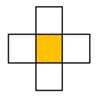
\includegraphics[width=20mm]{images/4_neigh.png} \\

	\item	
		8 points neighborhood \hspace{35pt}
			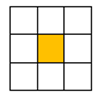
\includegraphics[width=20mm]{images/8_neigh.png} \\

	\item	
		24 points neighborhood \hspace{35pt}
			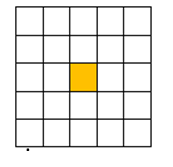
\includegraphics[width=20mm]{images/24_neigh.png} \\				
	\end{itemize}

\Large {\bf Pattern
} - is a combination of specific layout of cells on the grid and the set of rules to be applied for them.

\section{Description of requirements}

\hspace{15pt} The automaton will consist
of binary set of states (e.i. on / off) and will operate in 3 different environments:
\begin{itemize}
	\item 4 points neighborhood.
	\item 8 points neighborhood.
	\item 24 points neighborhood.
\end{itemize}
\par The application will allow user to create, save and edit rules based on this environments and of course observe each generation on the two dimensional finite in size grid of cells
(the grid will have wrapping option to simulate infinite size - the left edge will be connected with right edge).
\par The user will be able to draw cells on the grid and save the state of grid into patterns.
The user can easily move around the grid, zoom in and out.



\section{Description of requirements}



\section{User stories}
As... I want... because

\section{Evaluation of solution}


.
\\\\\\\\\\\\\\\\Introduction
	Purpose
	Definitions
	System overview
	References
	
Overall description
	Product perspective
		System Interfaces
		User Interfaces
		Hardware interfaces
		Software interfaces
		Communication Interfaces
		Memory Constraints
		Operations
		Site Adaptation Requirements
	Product functions
	User characteristics
	Constraints, assumptions and dependencies
	
Specific requirements
	External interface requirements
	Functional requirements
	Performance requirements
	Design constraints
		Standards Compliance
	Logical database requirement
	Software System attributes
		Reliability
		Availability
		Security
		Maintainability
		Portability
	Other requirements




\end{document}
